\documentclass[letterpaper, 12pt]{article}
\usepackage[round]{natbib}
\bibliographystyle{apalike}
\usepackage[margin=1in]{geometry}
\usepackage{enumitem}
\usepackage{csquotes}
\usepackage{graphicx}
\usepackage{float}
\usepackage{svg}


\usepackage{xcolor} % 
\newcommand{\bca}[1]{\textcolor{blue}{BCA: #1}} % Blair
\newcommand{\jl}[1]{\textcolor{purple}{JL: #1}} % Li
\newcommand{\todo}[1]{\textcolor{red}{#1}} % Things to fix.

\begin{document}
%\title{Proposal for the application to UTSC Postdoctoral Fellowship %Program}
%\author{Jiangtian Li}
%\maketitle

A central challenge in developing a theory of how the mind processes language is how the meanings of ambiguous words are resolved, given that about 85\% of the words in the world's languages are ambiguous \citep{KleinRepresentationPolysemousWords2001}.  For example, in the phrase ``A prime minister wields significant power'' a reader has no difficulty evoking a ``political power'' interpretation as opposed to an ``electrical power'' interpretation.  How this ambiguity is resolved remains an open question, despite having received attention from interdisciplinary researchers, and despite the game-changing role that a theory of ambiguity resolution could have for artificial intelligence. 

\bca{You are tight on space and information about the overview of the proposal is partially overlapping with the research plan idea.  I would merge those two points together to save space.  This will also help make some of the proposal points more concrete, as they are very abstract as they are currently phrased.}

My proposal builds upon the latest insights from several disciplines to develop a novel account of ambiguity resolution.  My philosophy background has made me appreciate the fundamental weakness of modeling a cognitive ability such as ambiguity resolution without grounding the model in knowledge of the external world \citep{harnadSymbolGroundingProblem1990, searleMindsBrainsPrograms1980}. \bca{cite one of these papers; you need to make a call on whether it is better to cite something old vs. newer, based on how impactful the work is.  Personally, I know the Searle work, but I don't know how representative my knowledg eon this front is}.  Second, I will adopt the view in cognitive science that understanding language fundamentally requires language to be part of a broader system for understanding and communicating about situations. \bca{it is unclear how point 1 is different than point 2 here.  Are they redundant?  If they are, maybe just leave point 1?}  Third, from the psycholinguistics and neuroscience literatures (including work by my proposed advisor, Professor Blair Armstrong), I will use a neurobiologically plausible architecture to constrain processing in ways that have been shown to improve the fit of the models to human behaviour \citep{Armstrong2016Disparatesemanticambiguity}.  

RESEARCH PLAN: My research plan starts from a (relatively) simple neural network model and gradually increasing the complexity of this model to understand how each addition impacts performance.  All of these models will be trained on databases of images and their associated captions, such as the COCO (Common Objects in Context) dataset, so that they, (except the first control model), learn to see objects while simultaneously processing their verbal description. Each model will be tested against ``gold standard'' published experimental data in the psycholinguistics literature that measures how quickly and accurately ambiguous words are resolved in different experimental tasks.  \bca{you may need a citation here to describe these data.  Perhaps the eddington and tokowicz review paper?}

1.  Language-only model. The first model will be trained only on text captions and will provide a baseline for how much disambiguating information can be extracted from text alone.  This approach is currently widespread in computational linguistics, and has been shown to contain substantial (although far from complete) disambiguating information. \citep{beekhuizenWhatCompanySemantically2018}

2.  Integrated vision-and-language model.  The second model will add a visual processing system to the model developed in (1), and will serve as a first validation for how visual information can provide additional constraint on word meaning than the prior model.

3.  More biologically plausible integrated model.  The third model will focus on how several key principles from cognitive and systems neuroscience could further enhance performance in the model: 3(a) Addition of an attention mechanism. Humans do not process all of the information their eyes take in equally well, rather, they focus attention on one part of the visual field and extract substantially more information from that area than others. 3(b) More realistic cortical connectivity.  In artificial neural networks, artificial neurons are typically able to send both positive (excitatory) and negative (inhibitory) information to other neurons, and often every neuron in one simulated brain area is connected to every neuron in another brain area.  In ``real'' neural networks, such as the human brain, neurons send excitatory OR inhibitory information, NOT both; there are vastly more ($\approx85\%$) excitatory neurons than inhibitory neurons ($\approx15\%$), and there are relatively few connections between different brain regions, such as vision and language. Prior work \citep{laszloPSPsERPsApplying2014, Armstrong2016Disparatesemanticambiguity} has established that these principles critically shape what type of information shapes network performance, including word disambiguation.  \bca{you can cut down this paragraph quite a bit, just condense the description of biologically plausible principles, maybe only highlighting some of them, or doing a higher-level overview of all of them}.   

EXPECTED OUTCOME AND IMPLICATIONS: I will revolutionize how ambiguity is thought about in many fields by merging insights from several fields to develop an account that would not emerge from any one discipline in isolation. \todo{revise here: Another implication is how abstract polysemous words are understood based on visual information. The political and ability senses of power are less connected to the physical world but people have been arguing that they share the same root as more physical words. This project will also serve as an attempt to test where the meanings of abstract polysemous words are rooted. }  \bca{the prior couple of sentences need to be revised.  It reads as a domain-specific list whose impact will be lost to a panel of experts, some who might noe even know what a polyseme is.  list specific fields / impacts, like you will show how language and vision need to be thought of as fundamentally intertwined constructs, not studied as seperate modules.  You need to end strong here, not on some weak note, or it will kill the application.  }  Finally, I aim to patent this model for use in artificial intelligence systems such as those used by Microsoft, Google, Facebook, etc. while allowing its free open-source use and development for academic purposes.  
\bca{moved from intro: you could merge this with the last sentence; you don't have space to be repetitive: Indeed, a firm grasp of the fundamental principles governing ambiguity resolution will revolutionize applications of language technologies including building better ``bots'' to communicate with customers online, and better automated screening of user content for remarks that are inappropriate or discriminatory.  }


\begin{figure}[h]
\begin{center}
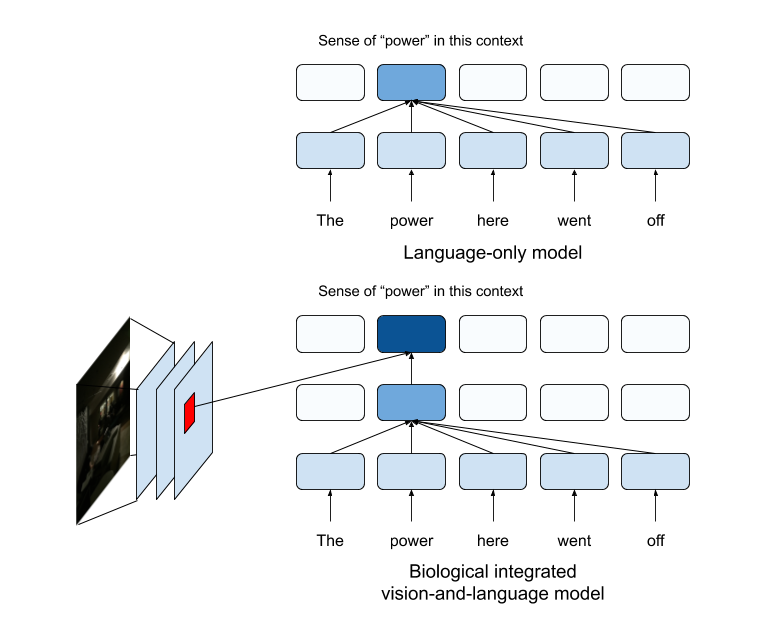
\includegraphics[width=0.7\textwidth,keepaspectratio]{model_figure}
\end{center}
    \caption{Computational models that are going to be build in this project.}
\end{figure}

\newpage
% \bibliography{/Users/jiangtianli/MyWriting/Mybib.bib}
\bibliography{Proposal_for_fellowship.bib}
\end{document}


\bca{The figure you have used would be ok for a domain-specific paper, but I suggest it needs to be reworked here.  I would not try to explain something like a convolutional network in this context, you might just want to show "visual input" with an actual picture of a power line" or similar.  Or maybe you want to pick an example where the sentence seems a bit ambiguous but would be fully resolved by the picture, so that you can give an intuition of the information in the image and how it will contribute to the process.  Second, you don't need to duplicate the top figure and the bottom figure, as this is very redundant and not efficient use of space for a one-page example.  You could instead just have one model.  If it were tractable, you could put boxes around each model to show how they relate to steps 1-3 above, but maybe that won't be practical.  You might consider something like the McClelland PNAS figure we discussed in his recent paper.  Perhaps something like having "language processing model" feeding onto a meaning representation, then a "vision model" feeding into that model, with both of them connecting to the meaning layer.  The weakness here is you can't show how the model is biologically plausible, so you'd have to give that intuition in the text.  You could consider just showing what one hidden layer looks like, maybe one standard big oval with little circles in it to show how they are artificial neurons, although maybe that will be too complex.  I would not show the full unrolling of the model over time, we'll just have to either gloss over that or have aquick comment about how the model will get the words one by one and estimate the meaning of the caption at each point in time.  It is a bit tricky too in that we have not given an intuition of what the task is doing (i.e., what the output representation looks like to give supervised learning).  Maybe the task is to try to generate the image sometimes from the text, and sometimes generate the text from an image, and use this as a mechanism for training the meaning layer to map between layers as in Rogers et al.'s hub and spoke model?}


\bca{not sure if you need references or not according to the instructions, or if you jst need citations}